%%%%%%%%%%%%%%%%%%%%%%%%%%%%
\section{Installation and Integration}
\label{sec:fdsp-hv-transport-install}
Installation of the components of the \dword{hvs} starts with the downstream (non-TCO end) \dwords{ewfc}.  Two endwall ``toaster'' crates   
%\fixme{They are toaster crates because the EndWall pieces are packed so that you can remove them one at a time like taking several pieces of toast out of a 4-slot toaster.  We decided to use crates that could be brought into the clean room and I think the idea is to wrap the toaster crates at the factory so that they are as clean as the Endwalls and can then go into the cryostat - SRM}
containing four endwall modules each, are transported into the cryostat.  Together they contain the eight individual modules that make up the  
downstream \dword{ewfc} for one drift volume.   


The modules are removed from their crates starting with the topmost unit and proceeding by attaching subsequent modules until the entire eight-module, \SI{12}{m} structure
is hanging vertically from its support beam.  This is repeated for the remaining three assemblies, making up the full downstream \dword{ewfc}. 
Figure~\ref{fig:EndwallInstall} shows a completed \dword{pdsp} endwall. 

Next, the first of the 25 rows of \dword{apa}s and \dword{cpafc} assemblies (counted lengthwise along the \dword{detmodule}) are positioned in the order \dword{apa}, \dword{cpafc}, \dword{apa}, \dword{cpafc}, \dword{apa}.  Electrical and mechanical connections between the \dword{ewfc} and \dword{apa}s and the \dword{ewfc} and \dword{cpa} arrays are made.  At this point, deployment (unfolding) of the \dwords{topfc} and \dwords{botfc} 
occurs.  Once they 
are latched at the \dword{apa} ends and 
the \dword{fc} termination connections are made and verified on the \dword{apa}s, this \dword{tpc} row is complete.  Subsequent rows of \dword{apa}s and \dword{cpafc} assemblies are positioned sequentially, using the same procedure, completing the 25 rows. 
Once the 25th row is in place, its \dword{topfc} is deployed, latching to the \dword{apa}s.  Before the \dword{topfc} is deployed, the upstream \dword{ewfc} crates are brought into the cryostat 
and the \dwords{ewfc} are built up from their crates in the same manner as the downstream ones.   
Once they  are in place and the \dwords{botfc} are deployed, the \dword{tpc} volume is enclosed. 
Finally, electrical and mechanical connections between \dwords{ewfc} and \dword{apa}s and between \dwords{ewfc} and \dword{cpa} arrays are made, completing all field cage connections in the \dword{tpc}.

%% added by BY
Compared with the time needed to install and verify the \dword{apa}s, the \dword{cpa}-\dword{fc} modules installation is relatively simple, using
the step-by-step installation procedures with associated checklists documented in~\cite{bib:docdb10452}.  The  procedures are based on the successful \dword{pdsp} experience.  
 Since the deployment of the top and bottom \dwords{fc} blocks physical access to the 
 enclosed volumes, the installation scheme described above limits the access to the installed \dword{tpc} components to only the outermost row being installed.  An alternative installation scheme that offers accessibility for a much longer period of time is under consideration.  In this scheme, after the far \dword{ewfc} is completed, both \dword{apa}s and \dword{cpa}/\dwords{fc} are installed into position along their DSS rails at their natural pace without deploying the \dwords{fc}. This leaves the aisles between the \dword{cpa}s and \dword{apa}s free with the floor in place in case access to previously installed \dword{tpc} modules is needed.  Once nearly all \dword{apa}s are installed, the floor boards are removed and \dwords{fc} are deployed.   

\begin{dunefigure}[ProtoDUNE-SP CPA plane before and after FC attachment]{fig:cpas-in-cryostat}{Left: Completed \dword{pdsp} \dword{cpa} plane ready for \dword{fc} attachment. Right: Two completed \dword{cpa}-\dword{fc} assemblies in the \dword{pdsp} cryostat. The top and bottom \dwords{fc} with their \dwords{gp} attached are visible to the right of the cathode plane in their folded pre-deployment position.}
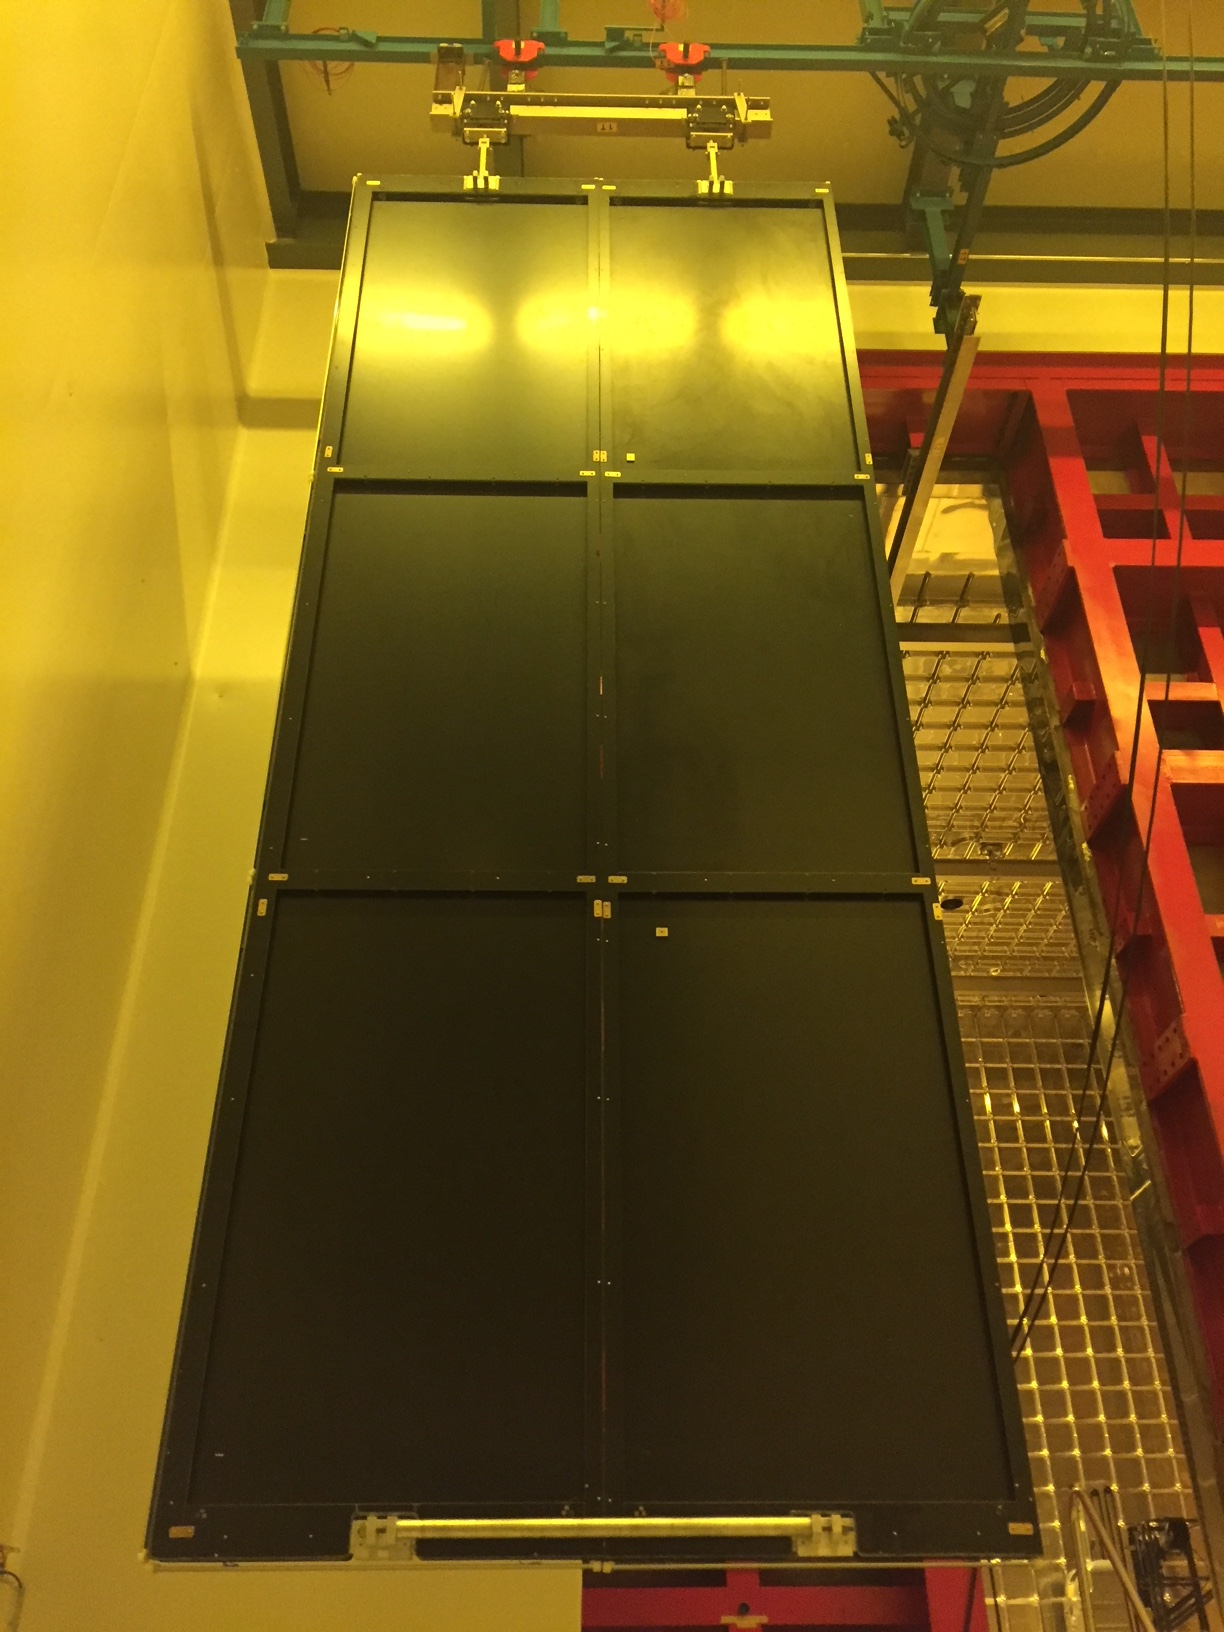
\includegraphics[width=0.45\textwidth]{lastcpa}
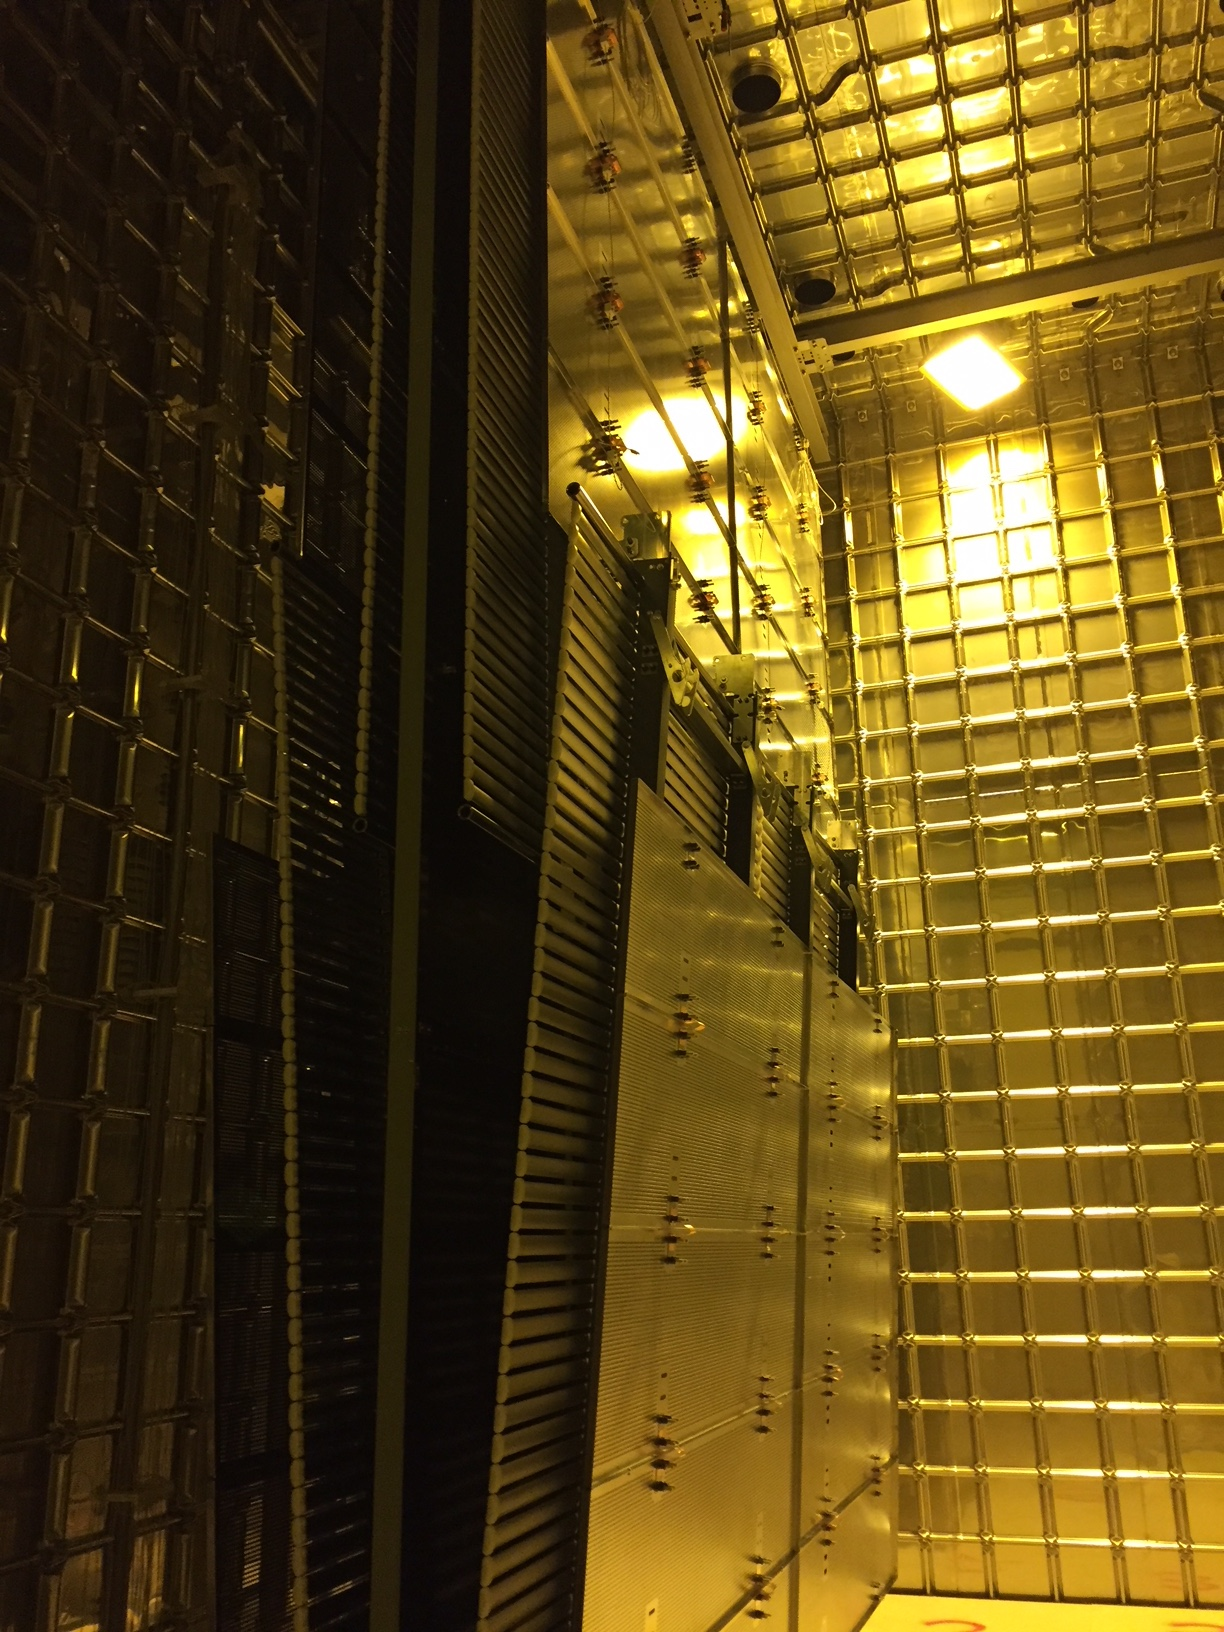
\includegraphics[width=0.45\textwidth]{2cpas-in-cryostat}
\end{dunefigure}

\begin{dunefigure}[ProtoDUNE-SP endwall FC installation]{fig:EndwallInstall}{Completed \dword{ewfc} during installation into the \dword{pdsp} cryostat. In
\dword{pdsp}, the individual endwall modules were connected to form the wall in the clean room before being pushed into the cryostat. 
For the \dword{spmod} the \dword{ewfc} will be built up inside the cryostat near its final position.}
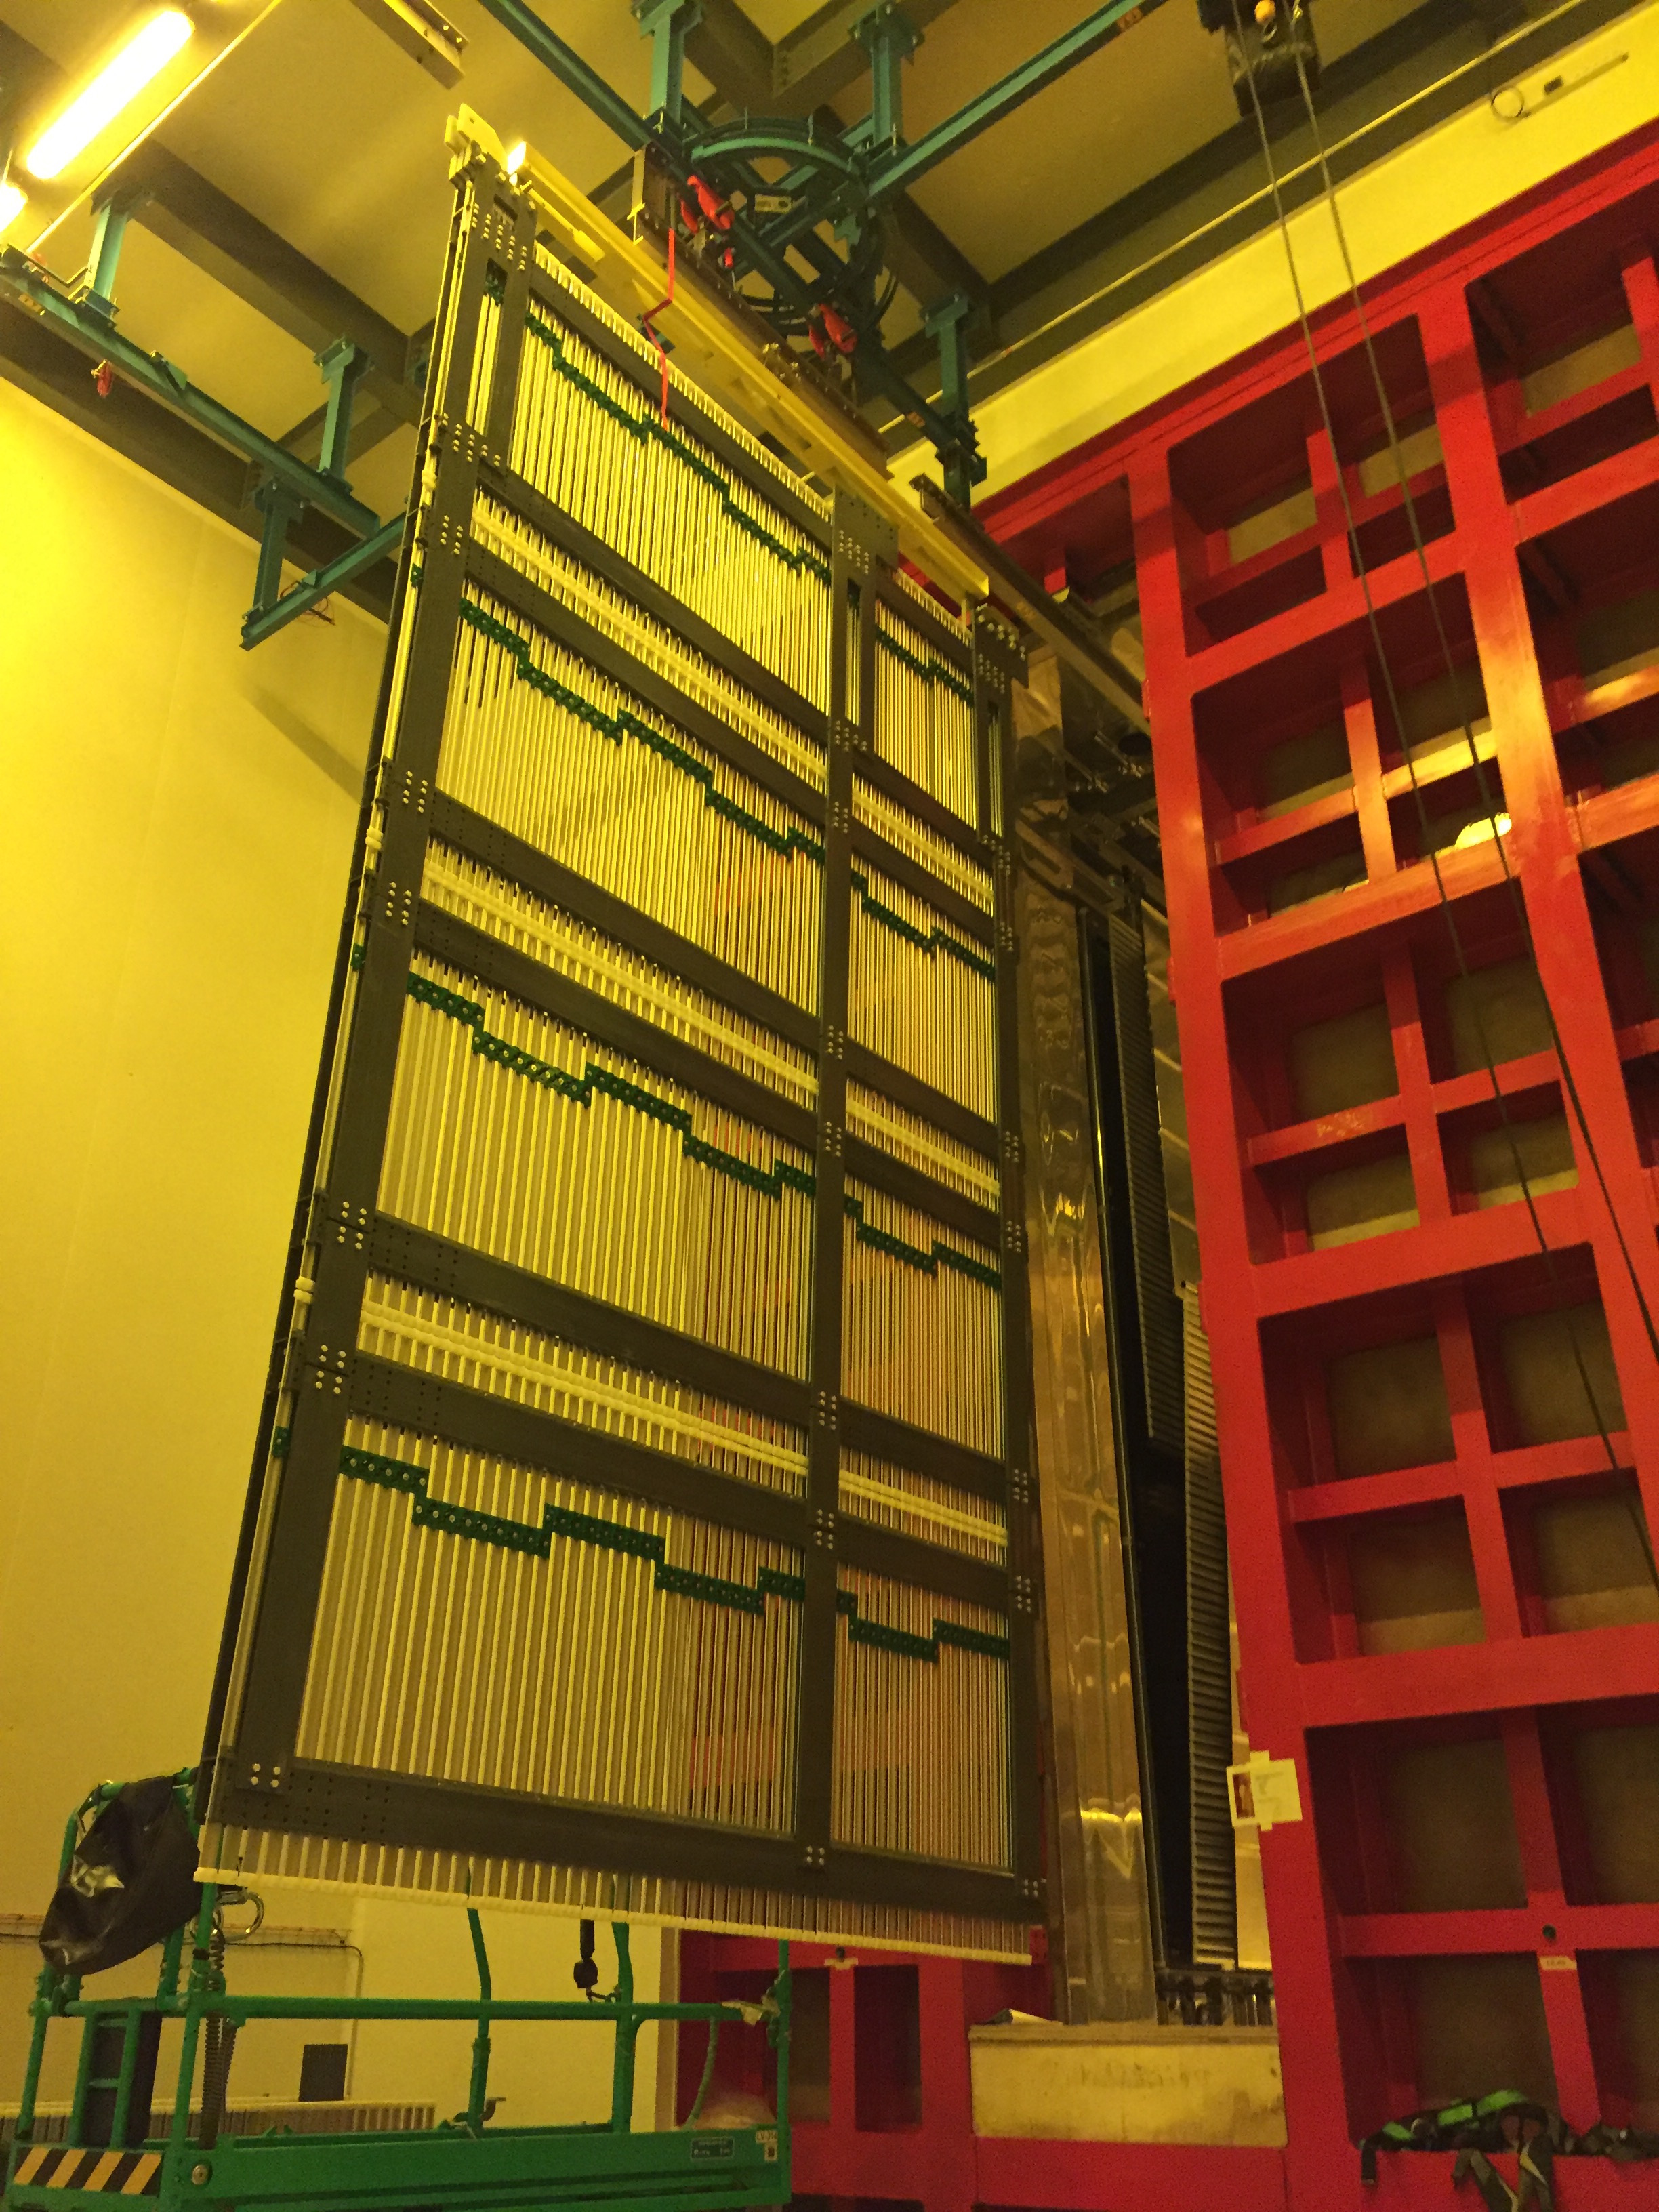
\includegraphics[width=0.65\textwidth]{endwall_and_tco.jpg}
\end{dunefigure}

